\documentclass{article}
\usepackage{amsmath}
\usepackage[utf8]{inputenc}
\usepackage{natbib}
\bibliographystyle{abbrvnat}
\setcitestyle{authoryear,open={((},close={))}}
\usepackage{graphicx}
\usepackage{float}
\usepackage[margin=1in]{geometry}
\usepackage{listings}
\lstset{language=Matlab}   




\title{MTH 5315 NUMERICAL METHODS FOR PDE \\ HOMEWORK 3}

\date{\today}
\author{\Huge Max L$\hat{\textrm{e}}$ \\ \\ ID: 901223283}
\begin{document}
\maketitle
\newpage
\tableofcontents
\newpage
\listoffigures
\newpage

\section{Introduction}
\subsection{Problem statement}
For this assignment, we are given the following 1D Poisson equation to solve: 
\\

\begin{equation}
u_{xx} = 1-2x^2
\end{equation}
\noindent
on the interval from 0 to 1. The boundary conditions are: $u'(0) = 1$ and $u(1) = 0$ at the ends. We are asked to solve the problem using three methods: Gauss Seidel,Conjugate Gradient Method without Preconditioner, and Conjugate Gradient Method with Incomplete Cholesky Decomposition until a residual error of $10^{-4}$ is obtained. The results are plotted and the convergent analysis is performed for each case. An analytical solution is also obtained via the following procedure: \\

\begin{align*}
u_{xx}(x) &= 1-2x^2 \\
\dfrac{d}{dx}(u_x(x))&= 1-2x^2\\
u_x(x)&= \int_{0}^{x} (1-2x^2) dx\\
&=x-\dfrac{2x^3}{3}+C1\\
u(x) &= \int_{0}^{x} (x-\dfrac{2x^3}{3}+C1) dx\\
&=\dfrac{x^2}{2} - \dfrac{x^4}{6} + C1x + C2
\end{align*}

\textrm{Applying the boundary conditions}

\begin{align*}
u(x) &=  \dfrac{x^2}{2} - \dfrac{x^4}{6} - \dfrac{1}{3}
\end{align*}
\subsection{Stencil}
In order to solve this PDE numerically, we must discretize it using a 2nd order central difference: 

\begin{equation*}
u_{xx} \approx \dfrac{u_{j+1}-2U_j+U_{j-1}}{\Delta x^2} + O(\Delta x^2)\\
\text{ for i = 1,2,..,N-1}
\end{equation*}

\noindent
This finite difference equation, when combine together with our original PDE, can be written in the form of a linear algebra system. 

\[
\dfrac{1}{\Delta x^2}\begin{bmatrix}
-2 & 1 & 0 & \dots & 0 \\
1 & -2 & 1 & \dots & 0 \\
0 & 1 & -2 & 1 & \dots \\
\dots  & \dots  & \dots  & \dots & \dots  \\
\dots & \dots & \dots & \dots & \dots 
\end{bmatrix}
\begin{bmatrix}
u_1 \\ u_2 \\ u_3 \\ \dots \\ u_n 
\end{bmatrix}
=
\begin{bmatrix}
f_1 \\ f_2 \\ f_3 \\ \dots \\ f_n 
\end{bmatrix}
\]

\noindent
This system can be written as: Au = f. Because our boundary condition requires Dirichlet at the end and Neumann at the front, we need to extend our grid by making ghost nodes.  The unknowns are now $U_0$ to $U_{N-1}$. For Neumann boundary conditions u'(x) = 0 = a, if we do a central difference, we would need a ghost point.  Let $U_{-1} = U_0 - h = -h$, then: 

\begin{align*}
	\dfrac{U_1 - U_{-1}}{2\Delta x^2} = a\\ 
	U_{-1} = U_1 - 2\Delta x^2 a
\end{align*}

\noindent
Recall the discretization that leads us to Au = f, we can write that equation again but at i = 0; 

\begin{equation*}
	U_{-1}-2U_0 + U_1 = \Delta x^2 f_0 
\end{equation*}

Substituting the equation for the ghost node into this with a = 0, we get:

\begin{equation*}
	\dfrac{1}{\Delta x^2}(-2U_0 + 2U_1) = f_0 
\end{equation*}

This means that the top level should have -2 and 2. Likewise, for the Dirichlet boundary condition, $U_N = 0 = b$, we write for i = N-1:

\begin{equation*}
	\dfrac{U_N-2U_{N-1}+U_{N-2}}{\Delta x^2} = f_{N-1}
\end{equation*}

\noindent
Rearranging, b = 0:

\begin{equation*}
	\dfrac{1}{\Delta x^2}(U_{N-2}-2U_{N-1}) = f_{N-1}
\end{equation*}

\noindent
This makes the last entry for $U_{n-1}$ to have a -2. Below is the revised system, with ghost points. 

\[
\dfrac{1}{\Delta x^2}\begin{bmatrix}
-2&2& 0 & 0 & \dots & 0 \\
0&1 & -2 & 1 & \dots & 0 \\
0&0 & 1 & -2 & 1 & \dots \\
\dots  & \dots  & \dots  & \dots & \dots & \dots  \\
\dots & \dots & \dots & \dots & \dots & -2
\end{bmatrix}
\begin{bmatrix}
u_0 \\ u_1 \\ u_2 \\ \dots \\ u_{n-1} 
\end{bmatrix}
=
\begin{bmatrix}
f_0 \\ f_1 \\ f_2 \\ \dots \\ f_{n-1} 
\end{bmatrix}
\]

\noindent
Our dx is calculated based on the following: $dx = \dfrac{xmax-xmin}{jmax-1}$. 

\newpage
\section{Gauss Seidel}

For this method, we assume that the matrix A can be decomposed into: A = L + U+D, where L = lower triangular matrix and U = upper triangular matrix and D = matrix whose diagonal belongs to A. Then, we can write: 

\begin{align*}
\vec{u}^{\,k+1} &= \vec{u}^{\,k} + \vec{B}^{\,-1}\vec{r}^{\,k}\\
 &= \vec{u}^{\,k} + (\vec{D}+\vec{L})^-1(\vec{f}-\vec{A}\vec{u}^k)\\
 &=(I-B^{-1}A)\vec{u}^{k} + B^{-1}\vec{f}
\end{align*}

\noindent
where B = L + D.  In our code, the matrix A is as follow: 

\[
A = \dfrac{1}{\Delta x^2}\begin{bmatrix}
-2&2& 0 & 0 & \dots & 0 \\
0&1 & -2 & 1 & \dots & 0 \\
0&0 & 1 & -2 & 1 & \dots \\
\dots  & \dots  & \dots  & \dots & \dots & \dots  \\
\dots & \dots & \dots & \dots & \dots & -2
\end{bmatrix}
\]

\noindent
The right hand side vector, or f, is as follow,following the function $1-2x^2$. This is only a sample because the actual size of the vector is 128x1

\[
f = \begin{bmatrix}
	1.000 \\ 0.999 \\ 0.995 \\ \dots \\ -0.9375 \\-0.9686 \\ -1.000 
\end{bmatrix}
\]
\newpage


\subsection{Results}

Below are results for this method: 


	\begin{figure}[H]
	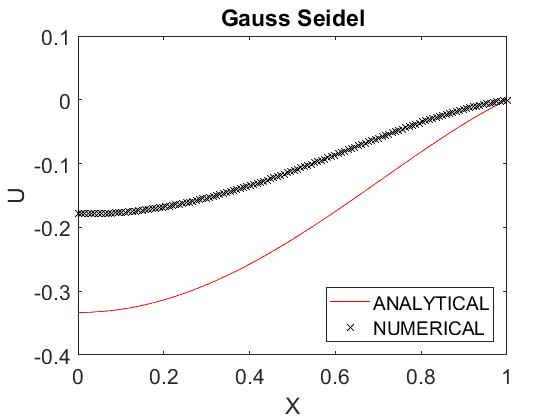
\includegraphics[width=\linewidth,height=80mm]{GS.jpg}
	
	
	\caption{Analytical vs Numerical Solution for Gauss Seidel method at 5000 iterations}
	\end{figure}

	\begin{figure}[H]
	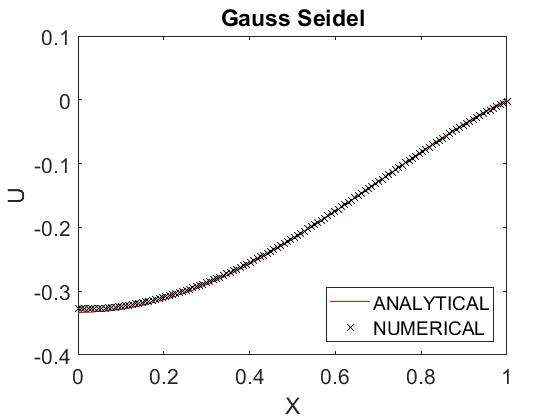
\includegraphics[width=\linewidth,height=80mm]{GS_50k.jpg}
	
	
	\caption{Analytical vs Numerical Solution for Gauss Seidel method at 50,000 iterations}
	\end{figure}


	The error distributions are plotted below for 5000 iterations and 50,000 iterations: 
	
	\begin{figure}[H]
		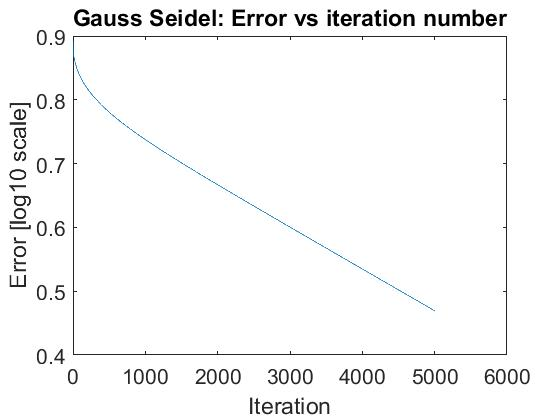
\includegraphics[width=\linewidth,height=80mm]{GS_error.jpg}	
		
		\caption{Error distribution for Gauss Seidel at 5000 iterations}
	\end{figure}


	\begin{figure}[H]
		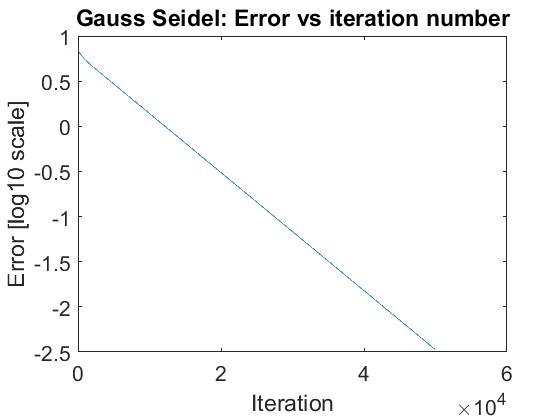
\includegraphics[width=\linewidth,height=80mm]{GS_error_50k.jpg}	
		
		\caption{Error distribution for Gauss Seidel at 50,000 iterations}
	\end{figure}

	\noindent
	We can see that in Figure 1, the numerical solution is getting closer to the analytical, however, it still needs more iterations to converge. In Figure 2, the result is very good because the numerical almost matches the analytical one. For the error distributions, we can see in Figure 3 that originally, the solution takes around 5000 iteration for the error to drop down.  At 50,000 iterations (Figure 4), we can see clearly, that higher iterations will help the solution to converge. At 50,000 iterations, the numerical solution can go down with error lower than 5000 iterations. This, of course, is only true if our initial guesses are not too far of from the analytical solution.
	
	  	

\subsection{Convergent Analysis}

Let $e_{k} = u - u_k$, where u is the exact solution and $u_k$ is the numerical solution. Then we can subtract the numerical solution from the exact solution to get the following error formula: 

\begin{equation}
u - u_{k+1} = (I-BA)(u-u_k) = (I-BA)(e_k) = (I-BA)^{k+1}e_0
\end{equation}

\noindent
For a residual corrective scheme, the convergence is only guaranteed if the spectral radius of the Residual Matrix is less than unity.  In other words: 

\begin{equation*}
\rho(I-BA) < 1
\end{equation*}

\noindent
For Gauss-Seidel, we have: $\rho(-(L+D)^{-1}U)<1$
\noindent
The spectral radius is the largest absolute eigenvalue of a matrix. In this case, we need to find the largest absolute eigenvalue of $(-(L+D)^{-1}U)$. This is performed by first calculating $(-(L+D)^{-1}U)$.  This is calculated in the code and is given the name \textbf{BGS}.  If this is a small matrix, then we would do: $det(BGS - \lambda I) = 0 $.  If we have a 3x3 matrix system, then to get the eigenvalues, we would need to solve a cubic polynomial. However, because we have a 128x128 system, the resulting polynomial would be of order 128th.  To solve this in MATLAB, the following command is used: 

\begin{align*}
\textbf{max(abs(eig(BGS)))}
\end{align*}

\noindent
The result is printed when the code is ran and is shown to be around 0.5002, which is less than 1.  Therefore, Gauss Seidel method, when apply to this system, guarantees convergent. This all depends on the requirement that A should be SPD (symmetric-positive-definite). In practice, the Gauss Seidel is used under a Successive Over Relaxation (SOR) form, where $w = 1$.  This form allows user to control the convergent rate of scheme. In the end, this shows that with given conditions, the Gauss Seidel method can give us a sequence approximating: $u^1, u^2,..., u^k$ that converges to the exact solution $u$. To see how fast this method works, we can use the following equation: 

\begin{equation}
	||u-u^k|| \leq ||B_{GS}||^k ||u-u_0||
\end{equation}

\noindent
From before, BGS = the iterative matrix and in the code, its norm is calculated by the variable \textbf{normBGS}, which is 0.740. If we exam the equation above, we can see that after each iteration, the error will decrease at a rate of $0.74^k$. The result is plotted below: 


\begin{figure}[H]
	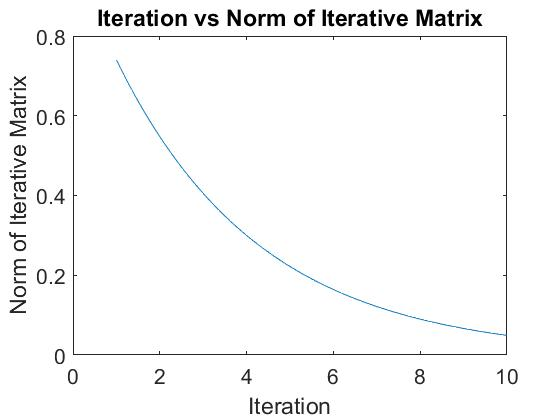
\includegraphics[width=\linewidth,height=80mm]{norm_plot_GS.jpg}	
	
	\caption{Iteration number vs Norm of Iterative Matrix}
\end{figure}

\noindent
This plot shows the rate at which the Iterative Matrix will go to zero. Form Equation 3, we can see that when $||B_{GS}^k$ is small, the term $||u-u^k||$ will be close to $||u-u0||$, making them to be close to each other. Another way to think about this is that the norm of Iterative Matrix acts similar to a limiter, that controls the error from the numerical solution and prevents it from increasing after each iteration.  


\section{Conjugate Gradient Method without Preconditioner}.  

\noindent
The idea behind the Conjugate Gradient (CG) method is that it employs a better search direction, in orthogonal direction, than in the Steepest Descent Algorithm (shown in the sample picture below). In other words,$p_k$ is calculated at each iteration based on the Gram-Schmidt conjugate. We can also think of this algorithm as approximating $u^k$ to the exact solution u, based on the initial residual $r0 = f-Au0$, or: 

\begin{equation*}
	u^k = u0+p0\alpha_0+...+p_{k-1}\alpha_{k-1}
\end{equation*}
\begin{center}
	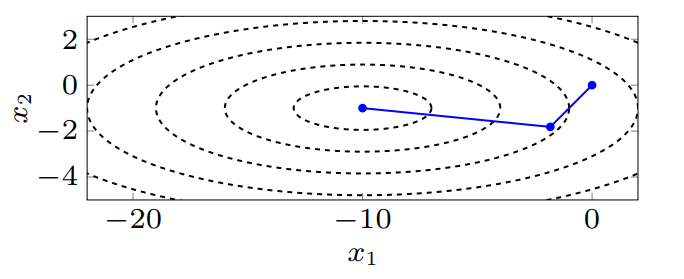
\includegraphics[scale=0.5]{search.png}
\end{center}

\subsection{Results}

Below are the results obtained from this method: 

\begin{figure}[H]
	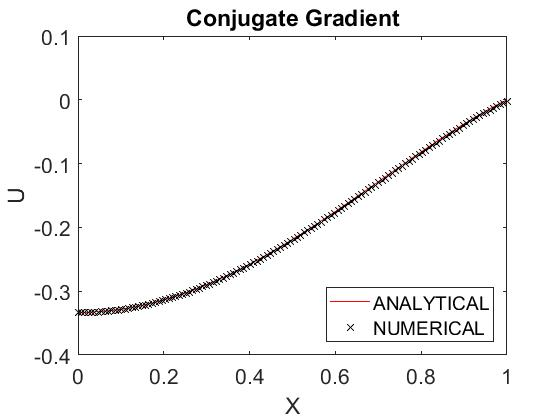
\includegraphics[width=\linewidth,height=80mm]{CG.jpg}
	\caption{Analytical vs Numerical Solution for Conjugate Gradient method at 1000 iterations}
\end{figure}

\begin{figure}[H]
	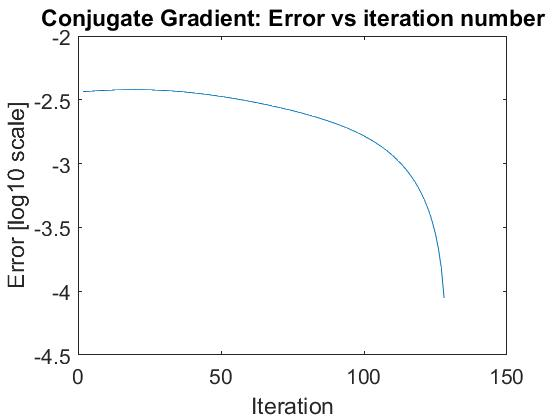
\includegraphics[width=\linewidth,height=80mm]{CG_error.jpg}
	\caption{Error distribution for Conjugate Gradient method at 1000 iterations}
\end{figure}

\noindent
We can see that overall, the magnitude of the error at each iteration is lower than Gauss Seidel. Gauss Seidel requires more than 50,000 iterations to converge and the error is around $10^{-1}$. Meanwhile, CG requires just around 120 iterations to converge and the error is much lower, around $10^{-3}$.   


\subsection{Convergent Analysis}

\noindent
We showed that in class, the relative error is bounded by:

\begin{equation}
	\dfrac{||u-u_k||_A^2}{||u-u_0||_A^2} \leq 2\left(\dfrac{\sqrt{\sigma }-1}{\sqrt{\sigma}+1} \right)^k
\end{equation}

\noindent
where k is the iteration number and $\sigma = \dfrac{\lambda max}{\lambda min}$ is the spectral conditioner.  We also need to recall the A-norm is defined as: 

\begin{equation}
	||g||_A = \sqrt{g^T A g}
\end{equation}

\noindent
We begin by taking the difference between numerical and analytical result, to get $u-u0$ and $u-u_k$.  This can shown in the code under the variables: \textbf{umu0} and \textbf{umuk}. Then, we applied the formula for the A-norm, and we get the following, where \textbf{normuksq} and \textbf{normu0sq} are the square norms in the MATLAB code. 

\begin{align*}
	||u-uk||_A^2 &=   -6.7029*10^{-6} \\
	||u-u0||_A^2 &= -0.0010
\end{align*}

\noindent
Thus, the left hand side of our relative error, is: $\dfrac{-6.7029*10^{-6}}{-0.0010} = 0.0065$

\noindent
To calculate eigenvalues, we use the MATLAB command: eig and we obtain the following: 

\begin{align*}
	\lambda max &= -1.5060*10^{-4} \\
	\lambda min &= -3.9998\\
	\sigma &= \dfrac{lambda max}{\lambda min} =  3.7650*10^{-5}
\end{align*}

\noindent
Substituting this into the RHS of our relative error equation with k = 128 iterations, we get: \\ $2\left(\dfrac{\sqrt{3.7650*10^{-5} }-1}{\sqrt{3.7650*10^{-5}}+1} \right)^{128} \approx 0.415$. 

\noindent
We can also take this a step further to verify that the following holds true: 

\begin{align*}
\dfrac{||u-u_k||_A}{||u-u_0||_A} &\leq \dfrac{1}{Tk\left(\dfrac{\lambda max + \lambda min}{\lambda max - \lambda min}\right)}
\end{align*}
\noindent
\textrm{Using MATLAB's Chebyshev command:} \\
\begin{align*}
0.0065 &\leq 0.3985
\end{align*}

\noindent
Therefore, we can say that with given linear system, which is obtained from a 2nd order central discretization, the relative error is bounded and the scheme converges. Of course, matrix A still needs to be SPD. Lastly, it is also important to note that, when the spectral radius increase to infinity i.e $\sigma \rightarrow \infty$ , then $\dfrac{\sqrt{\sigma }-1}{\sqrt{\sigma}+1} \approx 1- \dfrac{2}{\sqrt{\sigma}}$.  This result is a bigger (or faster) convergence rate if spectral radius is bigger than 1 if we compare this to Gauss Seidel's convergence rate at large spectral radius, which is $1- \dfrac{2}{\sigma}$


\section{Conjugate Gradient Method with Incomplete Cholesky Decomposition}

In order to improve the convergence of the CG method, we apply preconditioners to reduce the spectral radius of A. We then solve the transformed (with preconditioners), then we use the results obtained to solve a normal CG method. In this problem, we are asked to use Incomplete Cholesky Decomposition as the preconditioner.  This will give the transformed system: $Mz = r$, where $M = L^TL \approx A$. In order to get L, we use the following algorithm (from Wikipedia): 

\begin{figure}[H]
	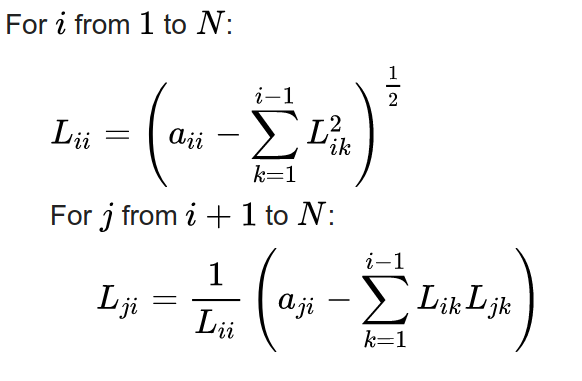
\includegraphics[width=60mm]{incomplete_cholesky.png}
\end{figure}

\noindent
The modified system ($Mz = r$) can be solved using any methods (Gaussian eliminations, LU decompositions..). In this problem, the modified system is solved using normal CG algorithm with its own tolerance: 

\begin{align*}
	Au &= f\\
	M^{-1}Au &= M^{-1}f\\
	(L^TL)^{-1}Au&=(L^TL)^{-1}f\\
	(L^T)^{-1}A(L^{-1})Lu &= (L^T)^{-1}f	\\
	\textrm{is equivalent to} \\
	\tilde{A}\tilde{u} &= \tilde{f}
\end{align*}



\noindent
The goal is to get the "tilda system" as starter for the main CG algorithm, so the tolerance is not a concern. Below are the results: 


\subsection{Results}


\begin{figure}[H]
	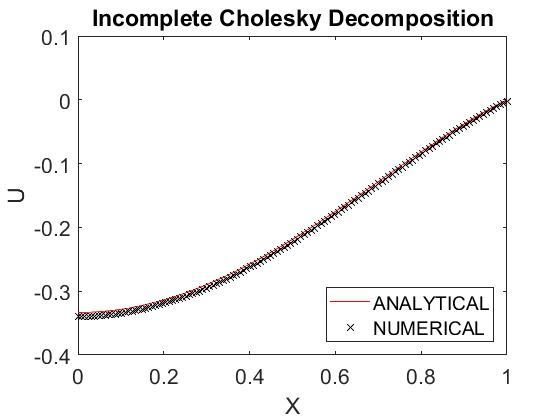
\includegraphics[width=\linewidth,height=80mm]{Cholesky_cg5.jpg}
	\caption{Conjugate Gradient method with Incomplete Cholesky Decomposition at 1000 iterations}	
\end{figure}


\begin{figure}[H]
	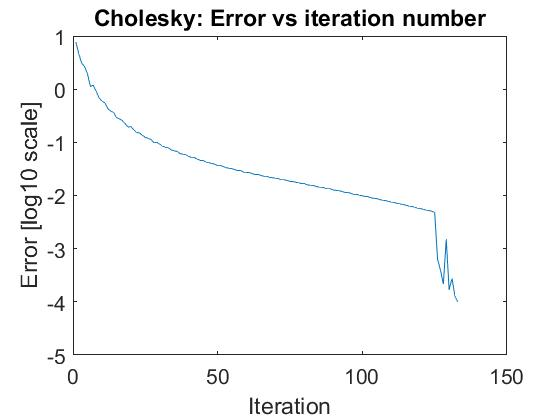
\includegraphics[width=\linewidth,height=80mm]{Cholesky_error_cg5.jpg}
	\caption{Conjugate Gradient method with Incomplete Cholesky Decomposition at 1000 iterations, z-tolerance = 5}	
\end{figure}

\begin{figure}[H]
	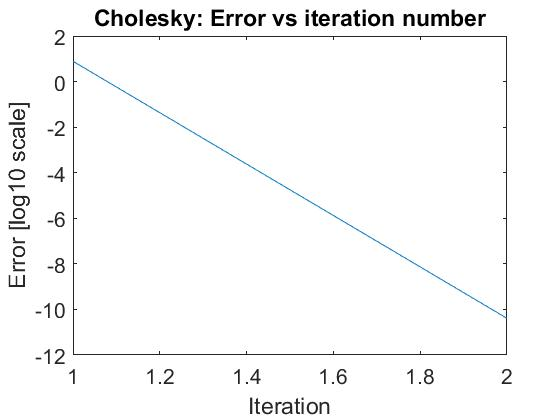
\includegraphics[width=\linewidth,height=80mm]{Cholesky_error_cg1e4.jpg}
	\caption{Conjugate Gradient method with Incomplete Cholesky Decomposition at 1000 iterations, z-tolerance = $10^{-4}$}	
\end{figure}

\noindent
Similar to the CG method, the numerical solution approaches the analytical solution at around 120 iterations. We can see from Figure 8, that the error does drop as iteration number goes up.  However, there are lots of fluctuations, especially at around 120-128 iterations, where the numerical solution reaches the required threshold. The reason for this could be that the modified system, $Mz = r$ is not solved correctly, and therefore the CG algorithm has to do more work or more iterations to keep the error down.  To investigate this, Figure 9 shows what happens if the tolerance for the modified system is set to be as low as $10^-4$: the scheme takes around 2 iterations to reach the required threshold.  Compare to CG method, the Incomplete Cholesky Decomposition is better if the modified system's tolerance is known.  Otherwise, we would have more iterations.  It is important to note that both the algorithms converge at the maximum grid size (128).  
\subsection{Convergent Analysis}
We apply the same relative error condition formula to this modified CG method: 
\begin{equation*}
	\dfrac{||u-u_k||_{\tilde{A}}^2}{||u-u_0||_{\tilde{A}}^2} \leq 2\left(\dfrac{\sqrt{\sigma }-1}{\sqrt{\sigma}+1} \right)^k
\end{equation*}

\noindent
The A-norm for both the errors are as follow. However, because we are dealing with a modified system, $\tilde{A}\tilde{u}=\tilde{f}$, the A-norm is actually the A*M norm. Again, the names are still \textbf{normuksq} and \textbf{normu0sq} in the MATLAB code. 
\begin{align*}
	||u-u_k||_{\tilde{A}}^2 &= 1.7498*10^3 \\
	||u-u_0||_{\tilde{A}}^2 &= 1.8928*10^3  \\
	\textrm{which gives the LHS to be}\\
	\dfrac{1.7498*10^3}{1.8928*10^3} &=  0.9245
\end{align*}

\noindent
The eigenvalues are now computed from the matrix: A*M, giving $\lambda max = 4.1611*10^9$ and $\lambda min =  5.8086$. This gives a spectral conditioner of $\sigma = 7.1636*10^8$. Substituting into the RHS of the relative error, we get: $2\left(\dfrac{\sqrt{7.1636*10^8 }-1}{\sqrt{7.1636*10^8}+1} \right)^{128} \approx 1.9810$. This threshold is higher than what we had for CG method;however, the relative error is still bounded (0.9245 < 1.9810). Therefore, this preconditioner with this particular system $Au = f$ for this particular discretized problem of the 1D Poisson converges with grid-size = 128. On the topic of grid size, we can also investigate the convergent rate by examining different grid size: 


\begin{figure}[H]
	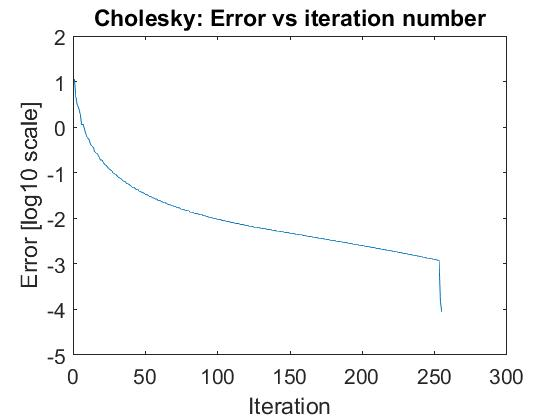
\includegraphics[width=\linewidth,height=80mm]{256.jpg}
	\caption{Conjugate Gradient method with Incomplete Cholesky Decomposition at grid-size = 256,z-tolerance = 5}	
\end{figure}

\begin{figure}[H]
	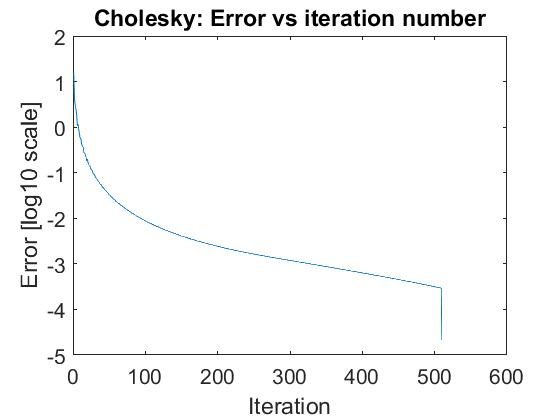
\includegraphics[width=\linewidth,height=80mm]{512.jpg}
	\caption{Conjugate Gradient method with Incomplete Cholesky Decomposition at grid-size = 512,z-tolerance = 5}	
\end{figure}

\noindent
We can see that at as the grid size double, there are less jagged lines on the error curves. One interesting thing to note is that both CG and CG with preconditioner stop at the specify grid size (i.e 128) in this case. 

\noindent
We can also try to plot the grid size with the norm of the error and see how it behaves. 

\begin{figure}[H]
	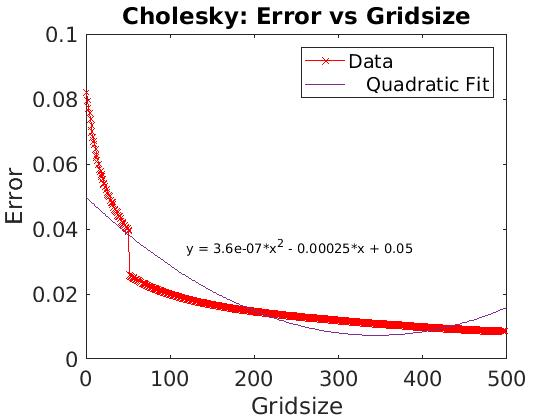
\includegraphics[width=\linewidth,height=100mm]{error_plot_CG.jpg}
	\caption{Conjugate Gradient method with Incomplete Cholesky Decomposition. Grid size vs Error}	
\end{figure}

\noindent
We can see that as the grid size increases, the error decreases and follow a parabolic path.  This makes sense because no matter what the tolerance of system is; we still have the original local truncation error of $O(\Delta x^2)$. If we have more grid points, our results would be more accurate and thus the error would decrease.  In this problem, because of our discretization, it decreases "parabolically". 

\newpage
\section{Conclusion}

The three methods: Gauss-Seidel, Conjugate Gradient method with and without Preconditioner all approach the analytical solution of our 1D Poisson equation. However, Gauss-Seidel requires the most iterations to converge (around 50,000).  On its own, the CG already converges faster than Gauss-Seidel (around 120 iteration).  If no informations are given about the solution of the modified linear system ($\tilde{A}\tilde{u}= \tilde{f}$), then the Preconditioner also converges at the same pace as CG (around 120 iterations). If the solution of the modified system is known, then a specific tolerance can be set and that accelerates the convergence of the secondary CG algorithm as well. In our code, it takes around 2 iterations for the CG algorithm to converge with a good tolerance for the modified linear system. \\

\noindent
In terms of convergent rate, the Gauss Seidel method, base on our analysis of the spectral radius, always converges. The Conjugate Gradient method and its preconditioner, based on the relative error analysis, are bounded by the required threshold. \\

\noindent
In terms of errors, the CG method's error distribution gets flattened out until around 100 iterations (Figure 6), then it drops and until it reaches the desire iteration to get a tolerance of $10^{-4}$.  Meanwhile, the Gauss-Seidel method takes longer for error to drop down to required tolerance (around 5000 iterations) in Figure 3. Lastly, the Incomplete Cholesky Decomposition does not get flattened out like the CG method.  Instead, it steadily drops until convergence is reached. The fluctuations from Figure 8 can be due to the errors from solving the modified linear system.  If the modified system is solve correctly, (or when the error is small), then there will be no fluctuations (Figure 9). Another way that we can think about this is that if the modified system is not correct, then the main CG algorithm would need more iterations to approach convergence.  Finally, we also need to bear in mind that the original PDE, after discretized into Au = f using second order central difference, will have an error of $O(\Delta x^2)$. This behavior of error is shown in Figure 13, where the error follows a parabolic path as grid size increases. 

\newpage
\section{Preference}

\begin{enumerate}
	\item Wikipedia-Cholesky Factorization. Web
	\item Class Notes MTH5315-Numerical Methods PDE. Florida Tech 
\end{enumerate}

\newpage

\section{Matlab Codes}
\subsection{GAUSS SEIDEL}

\lstinputlisting[language=MATLAB]{"/home/maxle/Dropbox/FIT GRAD MASTERS/SPRING 2018/NUM PDE/hw3/"max_le_gauss_seidel.m}
\newpage

\subsection{CONJUGATE GRADIENT WITHOUT PRECONDITIONER}

\lstinputlisting[language=Python]{"/home/maxle/Dropbox/FIT GRAD MASTERS/SPRING 2018/NUM PDE/hw3/"max_le_conj_gradient_no_Preconditioner.m}

\newpage

\subsection{CONJUGATE GRADIENT WITHOUT INCOMPLETE CHOLESKY DECOMPOSITION}

\lstinputlisting[language=Python]{"/home/maxle/Dropbox/FIT GRAD MASTERS/SPRING 2018/NUM PDE/hw3/"max_le_Cholesky.m}


\end{document}
